\section{Einleitung}

\begin{frame}
	\frametitle{Aktuelle Nachrichten}
	\only<1>{
		\begin{figure}
		\centering
		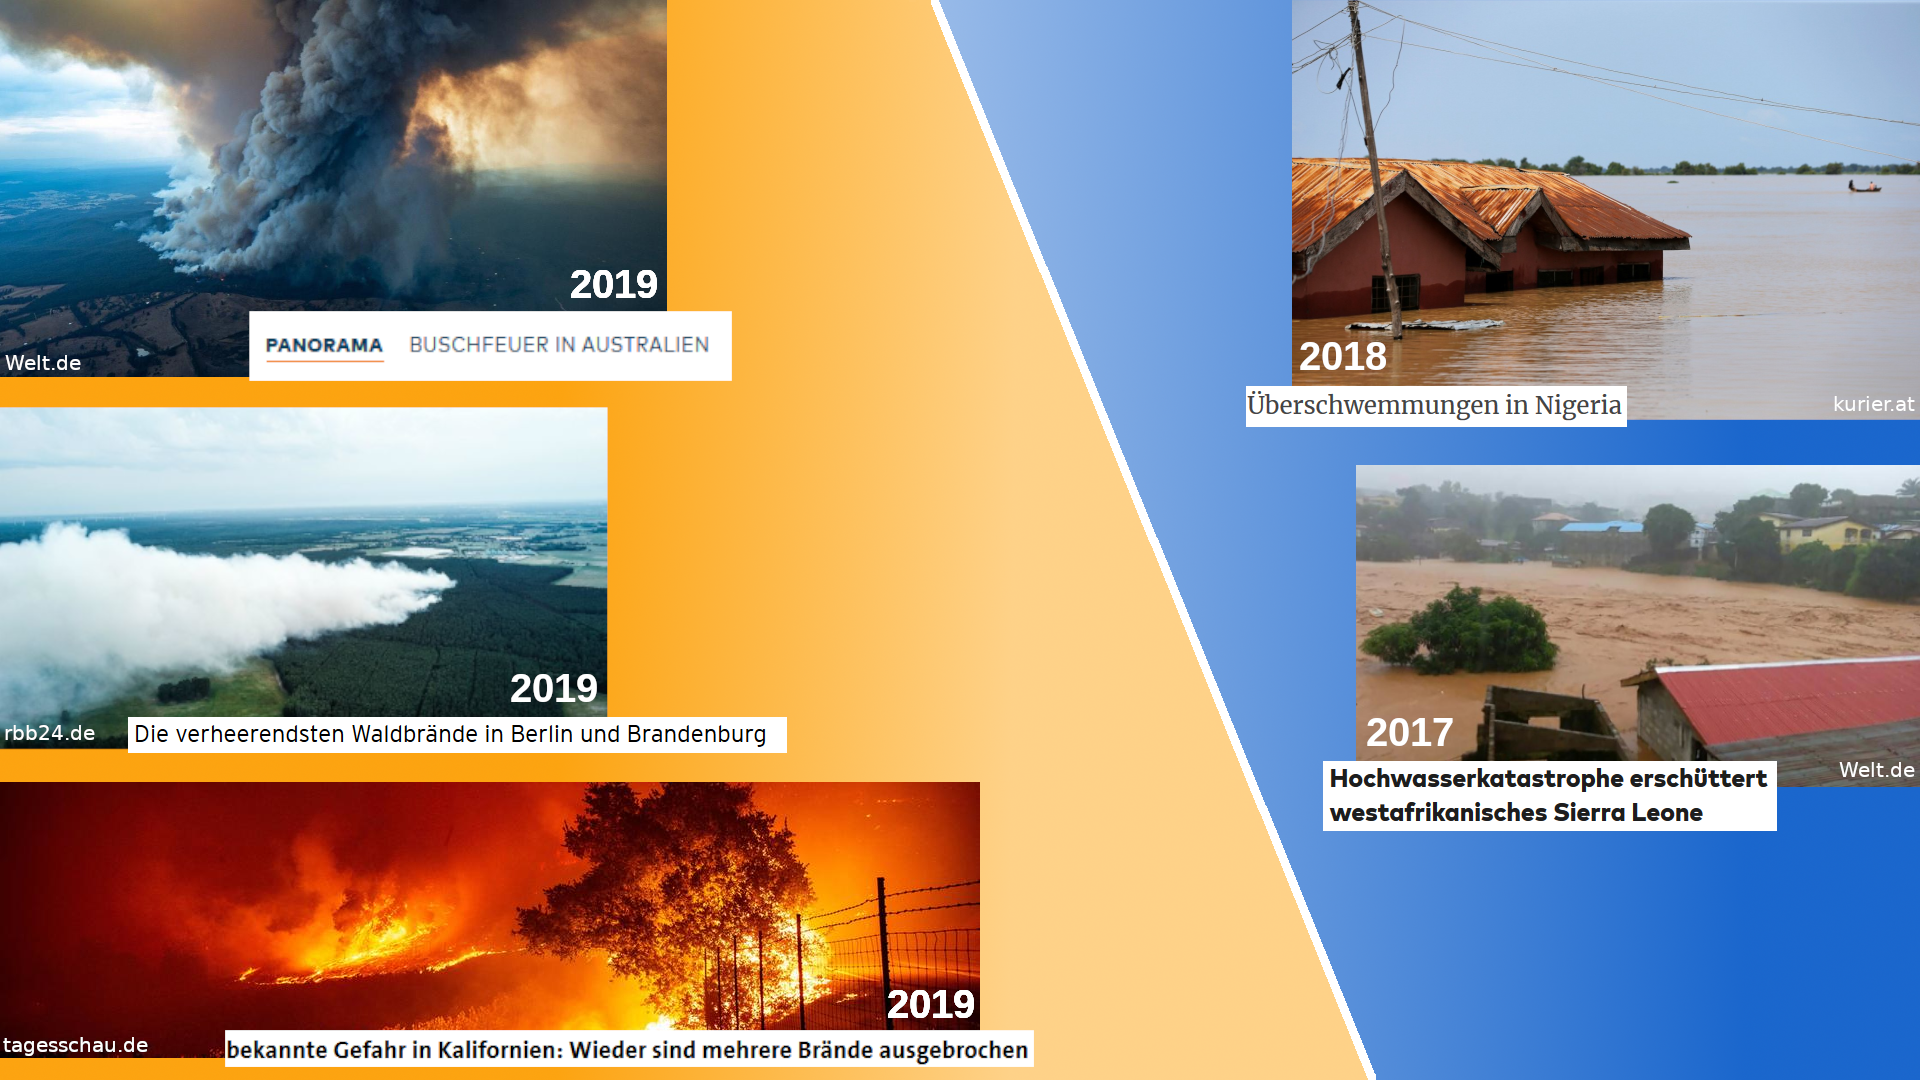
\includegraphics[width=0.9\linewidth]{bilder/CurrentSituation}
		\end{figure}
	}
	\only<2>{
	\begin{figure}
		\centering
		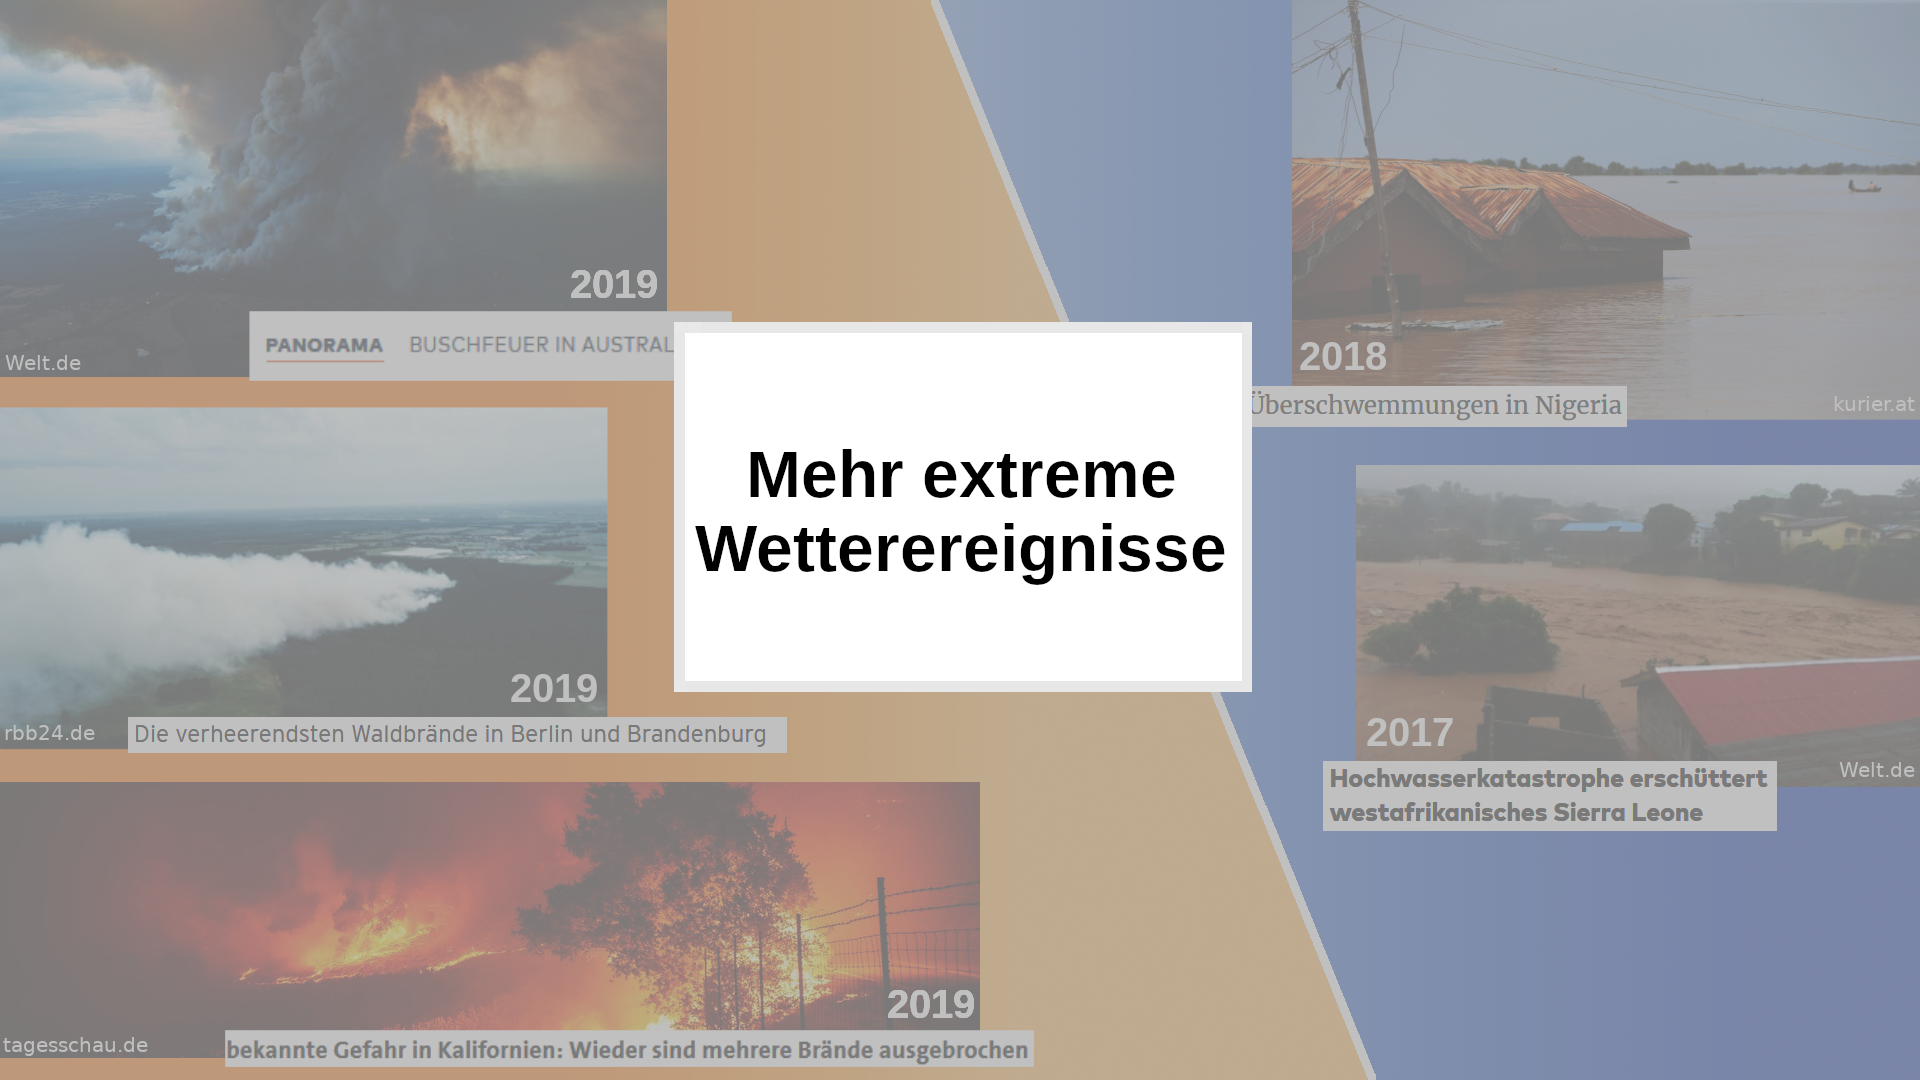
\includegraphics[width=0.9\linewidth]{bilder/CurrentSituation_Conclusion}
	\end{figure}
	}
	\only<3>{
	\begin{figure}
		\centering
		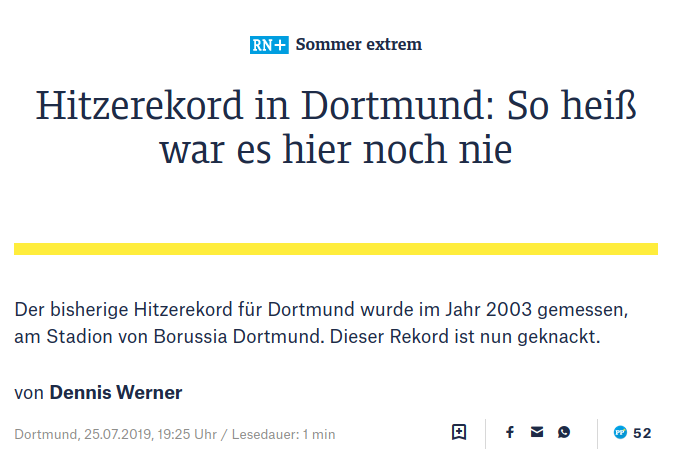
\includegraphics[width=0.5\linewidth]{bilder/dortmund}
	\end{figure}
	\begin{center}
		\textbf{Auch bei uns}
	\end{center}
	}

\end{frame}

% "es war doch immer schon im Sommer warm"


\begin{frame}
	\frametitle{Warming Stripes}
	% Abbildung der Warming Stripes: Die Entwicklung ist wirklich dramatisch
	
	% Farbskala erklären
	\begin{figure}
		\centering
		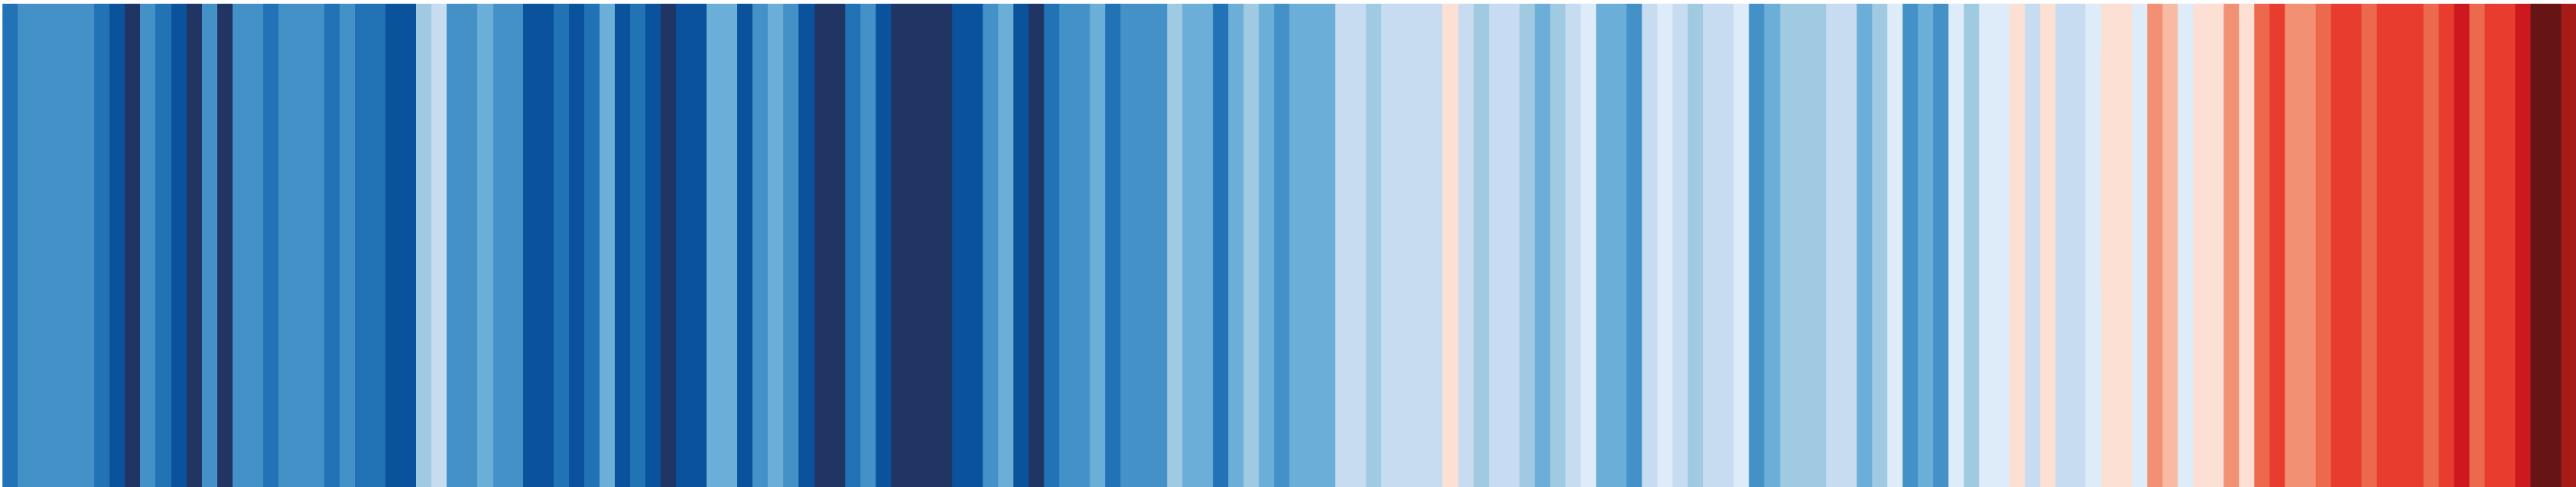
\includegraphics[width=\linewidth]{bilder/s4f-warming-stripes}
		\caption{Die \textit{Warming Stripes}}
		\label{fig:s4f-warming-stripes}
	\end{figure}
	\begin{itemize}
		\item Jeder Balken repräsentiert eine Jahr aus der Periode 1850-2017
		\item Blau = kälter als der Mittelwert, Rot=Wärmer
		\item Je dunklere die Farbe, desto extremer die Abweichung vom Mittelwert
		\item Die Trend geht klar zu höheren Temperaturen
		\item Übrigens auch das Logo der Scientists 4 Future
	\end{itemize}
\end{frame}

\begin{frame}
	\frametitle{Warming Stripes}
	% Extrapolation der Warming Stripes
	\begin{figure}
		\centering
		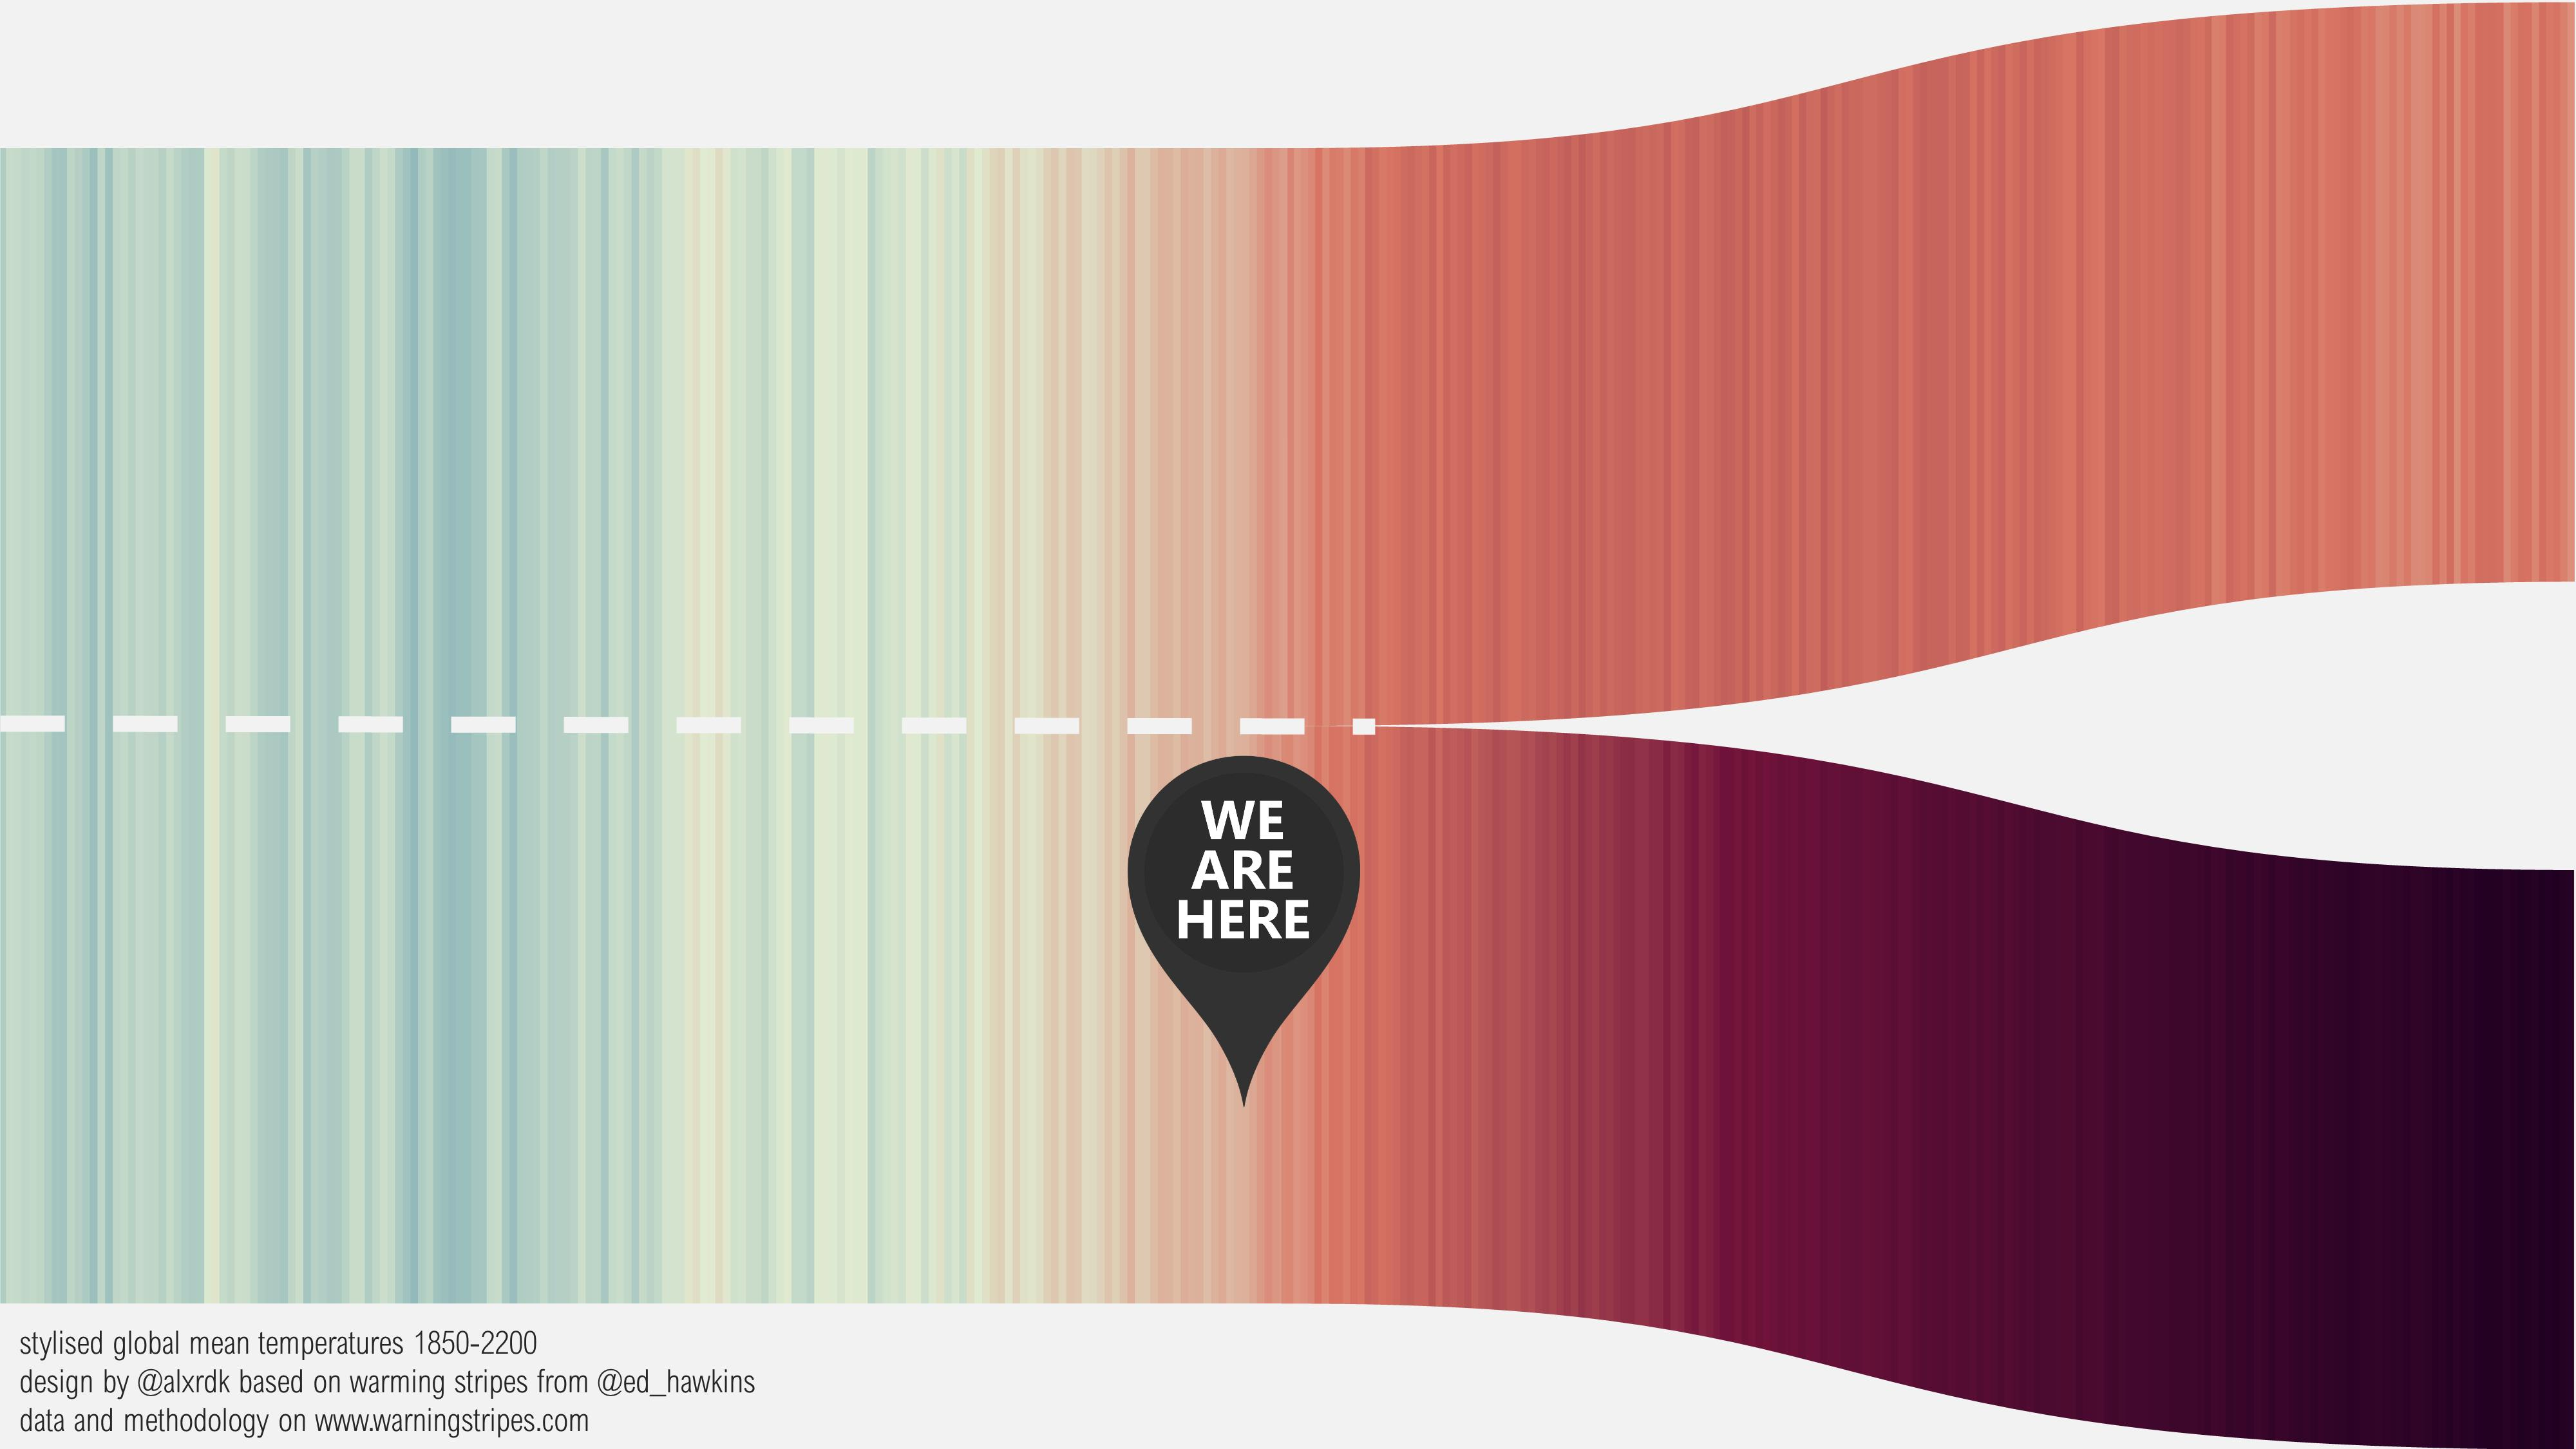
\includegraphics[width=0.6\linewidth]{bilder/warming_stripes_zukunft}
		\caption{Extrapolation der \textit{Warming Stripes} basierend auf Modellannahmen}
	\end{figure}
	\begin{itemize}
		\item In der Zukunft wird es sehr wahrscheinlich zu einer weiteren Erwärmung kommen
		\item Man kann statistische Prognosen für die Zukunft auf Basis von Modellrechnungen erstellen
		\item Der genaue Trend und die maximale Erwärmung hängen aber davon ab was wir heute und in den nächsten Jahren tun!
	\end{itemize}

\end{frame}